\documentclass[11pt]{article}

\usepackage[english]{babel}                 %% hyphenation rules, spell-checker
\usepackage{amsmath,amssymb}                        %% macros like align* and pmatrix
\usepackage{graphicx,epstopdf}              %% for .eps graphs
\usepackage[official]{eurosym}              %% 1 \euro
\usepackage[a4paper,margin=2cm]{geometry}   %% margins
\usepackage{hyperref}                       %% hyperlinks to urls
\usepackage{float}                    

\frenchspacing                              %% no extra space after period
\addtolength{\parskip}{0.5\baselineskip}    %% some white space between paragraphs
\setlength{\parindent}{0pt}                 %% but no indentation
\renewcommand{\baselinestretch}{1.1}        %% line spacing of TeX is small
\DeclareMathOperator{\E}{\mathbb{E}}
\DeclareMathOperator{\Var}{\text{Var}}
\DeclareMathOperator{\Cov}{\text{Cov}}


\title{Non-life --- Assignment NL2}  %% don't forget to change!

\author{
  Niels Keizer\footnote{Student number: 10910492}
  \quad and \quad
  Robert Jan Sopers\footnote{Student number: 0629049}
}

\date{\today}

\begin{document}

\maketitle

\section{Simulating an insurance portfolio-App. A3}

\subsection*{Q1}

How many bytes does it take to store $1,\ldots, 10, 1000, 100000$ logical values \verb|TRUE|/\verb|FALSE|?

We assume that $1,\ldots, 10$ means all the integers from 1 to 10. To how many bytes are needed in \verb|R|, we use the function \verb|object.size()|.

\begin{verbatim}
> for (n_values in c(1,2,3,4,5,6,7,8,9,10,1000,100000)){
+   hh <- rep(TRUE,n_values)
+   rr <- sample(c(TRUE,FALSE),n_values,repl=TRUE,prob=c(1,1))
+   af <- as.factor(rr)
+   print(c(n_values, object.size(hh), object.size(rr), object.size(af)))
+ }
[1]   1  48  48 464
[1]   2  48  48 464
[1]   3  56  56 528
[1]   4  56  56 528
[1]   5  72  72 544
[1]   6  72  72 488
[1]   7  72  72 544
[1]   8  72  72 544
[1]   9  88  88 560
[1]  10  88  88 560
[1] 1000 4040 4040 4512
[1] 100000 400040 400040 400512
\end{verbatim}

The first column of the output is the length of the vector. The second column indicates the size in bytes of a vector filled with only \verb|TRUE| values. The third with a random selection of \verb|TRUE| and \verb|FALSE|. The final column represents the size of the randomized vector, after it has been turned into a factor object.

\subsection*{Q2}

To obtain the \verb|y| vector, we first need to run the following code:

\begin{verbatim}
> n.obs <- 10000; set.seed(4)
> # n.obs <- 10000; set.seed(4) # Gebruik deze regel voor een grotere sample size.
> sx <- as.factor(sample(1:2, n.obs, repl=TRUE, prob=c(6,4)))
> jb <- as.factor(sample(1:3, n.obs, repl=TRUE, prob=c(3,2,1)))
> re.tp <- sample(1:9, n.obs, repl=TRUE, prob=c(.1,.05,.15,.15,.1,.05,.1,.1,.2))
> tp <- as.factor(c(1,2,3,1,2,3,1,2,3)[re.tp]) 
> re <- as.factor(c(1,1,1,2,2,2,3,3,3)[re.tp])
> mo <- 3 * sample(1:4, n.obs, repl=TRUE, prob=c(1,1,0,8))
> mu <- 0.05 * c(1,1.2)[sx] *
+              c(1,1,1)[jb] * 
+              c(1,1.2,1.44)[re] * 
+              1.2^(0:2)[tp] * mo/12 
> y <- rpois(n.obs, mu)
> table(y)
y
   0    1    2    3 
9276  702   20    2 
\end{verbatim}

Which is then inspected by calculating \verb|mean(y)|, \verb|var(y)| and the overdispersion factor \verb|var(y)|/\verb|mean(y)|.

\begin{verbatim}
> cbind(mean=mean(y),variance=var(y),phi=var(y)/mean(y))
       mean  variance       phi
[1,] 0.0748 0.0744124 0.9948182
\end{verbatim}

The overdispersion factor is smaller than $1$. This is possible because we are looking at a relatively small sample, with low probabilities. If we would take a much larger sample, the value would be larger than $1$. We check this by running the same code, but with a sample 100 times larger. This gives a result with an overdispersion factor larger than $1$.

\begin{verbatim}
> table(y)
y
     0      1      2      3      4 
931128  66053   2734     82      3 
> cbind(mean=mean(y),variance=var(y),phi=var(y)/mean(y))
         mean   variance      phi
[1,] 0.071779 0.07262285 1.011756
\end{verbatim}

\subsection*{Q3}

We create a dataframe by using the function \verb|aggregate()|.

\begin{verbatim}
> aggr <- aggregate(list(Expo=mo/12,nCl=y,nPol=1), list(Jb=jb,Tp=tp,Re=re,Sx=sx), sum)
\end{verbatim}

Then we compare the sizes.

\begin{verbatim}
> object.size(aggr) 
5336 bytes
> object.size(mo) 
80040 bytes
> object.size(y) 
40040 bytes
> object.size(jb) + object.size(tp) + object.size(re) + object.size(sx)
162240 bytes
\end{verbatim}

The amount of memory gained is equal to $80040 + 40040 + 162240 - 5336 = 276984$ bytes.

\subsection*{Q4}

According to MART Sec. 3.9.3, the maximum likelihood estimate $\hat{\lambda}_{3,3,3,2}$ is equal to the number of claims divided by the exposure.

\begin{verbatim}
> aggr[54,]
   Jb Tp Re Sx   Expo nCl nPol
54  3  3  3  2 115.75  13  130
> lambda3332 <- aggr$nCl[54]/aggr$Expo[54]
> lambda3332
[1] 0.112311
\end{verbatim}

In the first command, we show that observation 54 contains the desired aggregated values to calculate the estimate, which is then determined at $0.112$.

\section{Exploring the automobile portfolio of Sec. 9.5}

First we execute the following code in \verb|R| to generate the portfolio.

\begin{verbatim}
> rm(list=ls(all=TRUE)) 
> n <- scan(n=54) ## read 54 numbers into vector n
1:   1  8 10  8  5 11 14 12 11 10  5 12 13 12 15 13 12 24
19: 12 11  6  8 16 19 28 11 14  4 12  8 18  3 17  6 11 18
37: 12  3 10 18 10 13 12 31 16 16 13 14  8 19 20  9 23 27
Read 54 items
> expo <- scan(n=54) ## the number of policies 
1:  10 22 30 11 15 20 25 25 23 28 19 22 19 21 19 16 18 29
19: 25 18 20 13 26 21 27 14 16 11 23 26 29 13 26 13 17 27
37: 20 18 20 29 27 24 23 26 18 25 17 29 11 24 16 11 22 29
Read 54 items
> expo <- 7 * expo ## each policy is in force during a 7-year period
> sex <- gl(2,27); region <- gl(3, 9, 54); type <- gl(3, 3, 54); job <- gl(3, 1, 54)
\end{verbatim}

\subsection*{Q5}

We are asked to comment on the difference between to lines of \verb|R| code.

\begin{verbatim}
> str(type)
Factor w/ 3 levels "1","2","3": 1 1 1 2 2 2 3 3 3 1 ...
> str(rep(1:3, each=3, len=54))
int [1:54] 1 1 1 2 2 2 3 3 3 1 ...
\end{verbatim}

The \verb|str()| function compactly displays the structure of an arbitrary R object.
\verb|type| contains a \verb|Factor| object, with 3 ordered levels (or categories), and a list of integers which indicate which element is at that position.
\verb|rep(1:3, each=3, len=54)| creates a vector of integers of three ones, three twos and three threes, repeated to a length of 54.

\subsection*{Q6}

First we take a sample from a dataframe which contains the portfolio.

\begin{verbatim}
> set.seed(1); subset <- sort(sample(1:54,15))
> data.frame(sex, region, type, job, n, expo)[subset,]
sex region type job  n expo
3    1      1    1   3 10  210
8    1      1    3   2 12  175
10   1      2    1   1 10  196
11   1      2    1   2  5  133
15   1      2    2   3 15  133
16   1      2    3   1 13  112
20   1      3    1   2 11  126
29   2      1    1   2 12  161
30   2      1    1   3  8  182
31   2      1    2   1 18  203
32   2      1    2   2  3   91
45   2      2    3   3 16  126
46   2      3    1   1 16  175
47   2      3    1   2 13  119
48   2      3    1   3 14  203
\end{verbatim}

We are asked to check if the covariates of the first two cells have the right value. We print the right values of cells 3 and 8 using this code.

\begin{verbatim}
> cbind(sex=sex[3],region=region[3],type=type[3],job=job[3],n=n[3],expo=expo[3])
     sex region type job  n expo
[1,]   1      1    1   3 10  210
> cbind(sex=sex[8],region=region[8],type=type[8],job=job[8],n=n[8],expo=expo[8])
     sex region type job  n expo
[1,]   1      1    3   2 12  175
\end{verbatim}

We conclude that these are equal to those in the dataframe.

\subsection*{Q7}

We construct two analysis of deviance tables. One where \verb|type| is added before \verb|region| and the other way around.

\begin{verbatim}
> anova(glm(n/expo ~ type*region, quasipoisson, wei=expo))
Analysis of Deviance Table

Model: quasipoisson, link: log

Response: n/expo

Terms added sequentially (first to last)


            Df Deviance Resid. Df Resid. Dev
NULL                           53    104.732
type         2   36.367        51     68.365
region       2   23.424        49     44.940
type:region  4    2.529        45     42.412
> anova(glm(n/expo ~ region*type, quasipoisson, wei=expo))
Analysis of Deviance Table

Model: quasipoisson, link: log

Response: n/expo

Terms added sequentially (first to last)


            Df Deviance Resid. Df Resid. Dev
NULL                           53    104.732
region       2   21.597        51     83.135
type         2   38.195        49     44.940
region:type  4    2.529        45     42.412
\end{verbatim}

What we see is that the order in which these terms are added does not matter for the result. After both \verb|type| and \verb|region| are added, the resulting degrees of freedom and residual deviance is the same. We do of course see a difference between the analysis of only adding \verb|region| or \verb|type|.

\subsection*{Q8}

We are asked to explain the similarities and the differences between the following \verb|R| code.

\begin{verbatim}
> (g.wei <- glm(n/expo ~ region*type, poisson, wei=expo))

Call:  glm(formula = n/expo ~ region * type, family = poisson, weights = expo)

Coefficients:
  (Intercept)        region2        region3          type2          type3
     -2.98873        0.14988        0.42165        0.43376        0.45195
region2:type2  region3:type2  region2:type3  region3:type3  
     -0.08084       -0.02230        0.25559        0.10860  

Degrees of Freedom: 53 Total (i.e. Null);  45 Residual
Null Deviance:	    104.7 
Residual Deviance: 42.41 	AIC: Inf
There were 50 or more warnings (use warnings() to see the first 50)
> (g.off <- glm(n ~ 1+region+type+region:type+offset(log(expo)),
+               family=poisson(link=log)))

Call:  glm(formula = n ~ 1 + region + type + region:type + offset(log(expo)), 
    family = poisson(link = log))

Coefficients:
  (Intercept)        region2        region3          type2          type3
     -2.98873        0.14988        0.42165        0.43376        0.45195
region2:type2  region3:type2  region2:type3  region3:type3  
     -0.08084       -0.02230        0.25559        0.10860  

Degrees of Freedom: 53 Total (i.e. Null);  45 Residual
Null Deviance:	    104.7 
Residual Deviance: 42.41 	AIC: 290.7
\end{verbatim}

The output of \verb|g.off| and \verb|g.wei| contain the same coefficients, degrees of freedom, null deviance and residual deviance.
The AIC for g.off is 290.7, however, for g.wei this is Inf. Also, g.wei throws warnings, on further inspection these arise from having non-integer x values in calls to dpois. This is what prevents the \verb|glm| function from computing the AIC.

\subsection*{Q9}

We define the dummy functions \verb|region2| and \verb|type3| as follows:

\begin{equation}
\verb|region2| = 
\begin{cases}
	1 & \verb|region| = 2 \\
	0 & \verb|region| \neq 2
\end{cases}
\end{equation}
\begin{equation}
\verb|type3| = 
\begin{cases}
1 & \verb|type| = 3 \\
0 & \verb|type| \neq 3
\end{cases}
\end{equation}

Multiplying these functions gives a new function

\begin{equation}
\verb|region2| \cdot \verb|type3| = 
\begin{cases}
1 & \verb|region| = 2 \land \verb|type| = 3 \\
0 & \verb|region| \neq 2 \lor \verb|type| \neq 3
\end{cases}
\end{equation}

Here $\land$ is the logical AND operator and $\lor$ is the logical OR operator. We see that this function equals $1$ when \verb|region| equals $2$ and \verb|type| equals $3$, zero otherwise. It is therefore the same function as the dummy function \verb|region2:type3|.

\subsection*{Q10}

We run the following \verb|R| code to generate \verb|g.main|.

\begin{verbatim}
> g.main <- glm(n/expo ~ region+type, quasipoisson, wei=expo)
> coef(g.main)
(Intercept)     region2     region3       type2       type3 
-3.0313238   0.2314097   0.4604585   0.3941889   0.5833108 
\end{verbatim}

\subsubsection*{a)}

If $\verb|region|=1$ and $\verb|type|=1$, then the indicators for \verb|region2|, \verb|region3|, \verb|type2| and \verb|type3| are $0$. Thus we only have to calculate:
\begin{verbatim}
> exp(g.main$coefficients["(Intercept)"])
(Intercept) 
0.04825172 
\end{verbatim}

The first row of the dataset has region=1 and type=1, so we check against the fitted values from the glm.
\begin{verbatim}
> g.main$fitted.values[1]
1 
0.04825172 
\end{verbatim}

Which is the same.

\subsubsection*{b)}

We run the following code to determine the worst \verb|type/region| combination.

Assuming all \verb|type/region| combinations already exist in the model data (which is true):
\begin{verbatim}
> max(g.main$fitted.value)
[1] 0.1370301
\end{verbatim}

By going through all possible combinations using a max function:
\begin{verbatim}
> exp(g.main$coefficients[1]+max(0,g.main$coefficients[2:3])+max(0,g.main$coefficients[4:5]))
(Intercept) 
0.1370301 
\end{verbatim}
The maximum with $0$ is taken in case both coefficients for \verb|region| and/or \verb|type| are negative. In that case, the baseline $\verb|region|=1$ and/or $\verb|type|=1$ would be the worst case.

Showing all possible combinations:
\begin{verbatim}
> exp(g.main$coefficients[1]+matrix(c(0,g.main$coefficients[2:3]),3,3)
+                           +t(matrix(c(0,g.main$coefficients[4:5]),3,3)))
           [,1]       [,2]       [,3]
[1,] 0.04825172 0.07156602 0.08646522
[2,] 0.06081528 0.09020005 0.10897864
[3,] 0.07646934 0.11341785 0.13703011
\end{verbatim}

All three methods show that the estimated annual number of claims for the worst \verb|type/region| combination equals $0.1370301$. The third method shows that this is the case when $\verb|region|=3$ and $\verb|type|=3$.

\subsection*{Q11}

Here we reconstruct the vector of fitted values using \verb|R|. We also compare the results to the results from the model itself to show that the calculation is correct.

\begin{verbatim}
> cbind(g.off$family$linkinv(model.matrix(g.off) %*% coef(g.off) + g.off$offset),
+       fitted.values(g.off))
        [,1]      [,2]
1   3.524590  3.524590
2   7.754098  7.754098
3  10.573770 10.573770
4   5.982456  5.982456
5   8.157895  8.157895
6  10.877193 10.877193
7  13.846154 13.846154
8  13.846154 13.846154
9  12.738462 12.738462
10 11.464567 11.464567
11  7.779528  7.779528
12  9.007874  9.007874
13 11.071942 11.071942
14 12.237410 12.237410
15 11.071942 11.071942
16 13.292308 13.292308
17 14.953846 14.953846
18 24.092308 24.092308
19 13.432836 13.432836
20  9.671642  9.671642
21 10.746269 10.746269
22 10.540541 10.540541
23 21.081081 21.081081
24 17.027027 17.027027
25 25.411765 25.411765
26 13.176471 13.176471
27 15.058824 15.058824
28  3.877049  3.877049
29  8.106557  8.106557
30  9.163934  9.163934
31 15.771930 15.771930
32  7.070175  7.070175
33 14.140351 14.140351
34  7.200000  7.200000
35  9.415385  9.415385
36 14.953846 14.953846
37  8.188976  8.188976
38  7.370079  7.370079
39  8.188976  8.188976
40 16.899281 16.899281
41 15.733813 15.733813
42 13.985612 13.985612
43 19.107692 19.107692
44 21.600000 21.600000
45 14.953846 14.953846
46 13.432836 13.432836
47  9.134328  9.134328
48 15.582090 15.582090
49  8.918919  8.918919
50 19.459459 19.459459
51 12.972973 12.972973
52 10.352941 10.352941
53 20.705882 20.705882
54 27.294118 27.294118
\end{verbatim}

\subsection*{Q12}

We run the code from the assignment to get the following in \verb|R|.

\begin{verbatim}
> g. <- glm(n/expo ~ as.numeric(region)+type, quasipoisson, wei=expo)
> summary(g.main); summary(g.)

Call:
glm(formula = n/expo ~ region + type, family = quasipoisson, 
    weights = expo)

Deviance Residuals: 
     Min        1Q    Median        3Q       Max  
-1.92326  -0.65638  -0.05731   0.47902   2.31440  

Coefficients:
            Estimate Std. Error t value Pr(>|t|)    
(Intercept) -3.03132    0.09612 -31.537  < 2e-16 ***
region2      0.23141    0.09379   2.467 0.017149 *  
region3      0.46046    0.09135   5.041 6.73e-06 ***
type2        0.39419    0.09610   4.102 0.000154 ***
type3        0.58331    0.09191   6.347 6.82e-08 ***
---
Signif. codes:  0 ‘***’ 0.001 ‘**’ 0.01 ‘*’ 0.05 ‘.’ 0.1 ‘ ’ 1

(Dispersion parameter for quasipoisson family taken to be 0.8965432)

    Null deviance: 104.73  on 53  degrees of freedom
Residual deviance:  44.94  on 49  degrees of freedom
AIC: NA

Number of Fisher Scoring iterations: 5


Call:
glm(formula = n/expo ~ as.numeric(region) + type, family = quasipoisson, 
    weights = expo)

Deviance Residuals: 
     Min        1Q    Median        3Q       Max  
-1.92136  -0.65658  -0.05655   0.48053   2.31810  

Coefficients:
                   Estimate Std. Error t value Pr(>|t|)    
(Intercept)        -3.26097    0.12181 -26.770  < 2e-16 ***
as.numeric(region)  0.23014    0.04483   5.133 4.68e-06 ***
type2               0.39425    0.09507   4.147  0.00013 ***
type3               0.58332    0.09099   6.411 5.01e-08 ***
---
Signif. codes:  0 ‘***’ 0.001 ‘**’ 0.01 ‘*’ 0.05 ‘.’ 0.1 ‘ ’ 1

(Dispersion parameter for quasipoisson family taken to be 0.8787113)

    Null deviance: 104.732  on 53  degrees of freedom
Residual deviance:  44.941  on 50  degrees of freedom
AIC: NA

Number of Fisher Scoring iterations: 5

> anova(g., g.main)
Analysis of Deviance Table

Model 1: n/expo ~ as.numeric(region) + type
Model 2: n/expo ~ region + type
  Resid. Df Resid. Dev Df  Deviance
1        50     44.941             
2        49     44.940  1 0.0002148
\end{verbatim}

The residual deviances are pretty much equal, which means that both models are about equally as good at estimating the portfolio.

\verb|g.| is a restriction of \verb|g.main|, because by choosing \verb|region| to be numeric, you assume that the linear estimator for region $3$ is twice as big as the linear estimator for region $2$. So instead of having two degrees of freedom, you assume that there is a dependency between regions $2$ and $3$, which reduces the number of degrees of freedom by 1.

When you look at the region coefficients of \verb|g.main|, you see that the coefficient for region $3$ is indeed twice as large as the one for region $2$. Therefore this appears to make sense. However, there is no inherent order to regions, which means that the model should give the same results when we switch regions $2$ and $3$. $2$ and $3$ might as well be "Amsterdam" and "The Hague", the numbers are labels and not to be interpreted as actual ordered numbers. The \verb|g.main| model would simply switch the coefficients for the regions, but the \verb|g.| model would give different results. So while the restriction seems to make sense, it actually does not make sense at all, because it is an artifact of the ordering choice of the regions.


\subsection*{Q13}
We run the code from the question and obtain the following output:

\begin{verbatim}
> rm(list=ls(all=TRUE))
> n.obs <- 10000; set.seed(4) ## 10000 obs.; random seed initialized to 4
> sx <- sample(1:2, n.obs, repl=TRUE, prob=c(6,4)); sx <- as.factor(sx)
> jb <- as.factor(sample(1:3, n.obs, repl=TRUE, prob=c(3,2,1)))
> re.tp <- sample(1:9, n.obs, repl=TRUE, prob=c(2,1,3,3,2,1,2,2,4))
> tp <- as.factor(c(1,2,3,1,2,3,1,2,3)[re.tp])
> re <- as.factor(c(1,1,1,2,2,2,3,3,3)[re.tp])
> rm(re.tp)
> mo <- 3 * sample(1:4, n.obs, repl=TRUE, prob=c(1,1,0,8))
> mu <- 0.05 * c(1,1.2)[sx] * c(1,1,1)[jb] *
+   c(1,1.2,1.44)[re] * c(1,1.2,1.44)[tp] * mo/12
> y <- rpois(n.obs, mu)
> aggr <- aggregate(list(Expo=mo/12,nCl=y,nPol=1),
+                   list(Jb=jb,Tp=tp,Re=re,Sx=sx), sum)
> anova(glm(nCl~(Tp+Re+Sx+Jb)^4, poisson, offset=log(Expo), data=aggr), test="Chisq")
Analysis of Deviance Table

Model: poisson, link: log

Response: nCl

Terms added sequentially (first to last)


            Df Deviance Resid. Df Resid. Dev  Pr(>Chi)    
NULL                           53    101.825              
Tp           2   34.026        51     67.799 4.086e-08 ***
Re           2   20.075        49     47.724 4.374e-05 ***
Sx           1    3.565        48     44.159   0.05899 .  
Jb           2    1.438        46     42.721   0.48724    
Tp:Re        4    2.223        42     40.498   0.69477    
Tp:Sx        2    4.612        40     35.886   0.09967 .  
Tp:Jb        4    3.513        36     32.373   0.47588    
Re:Sx        2    0.795        34     31.578   0.67189    
Re:Jb        4    6.295        30     25.283   0.17818    
Sx:Jb        2    2.746        28     22.537   0.25333    
Tp:Re:Sx     4    1.780        24     20.757   0.77619    
Tp:Re:Jb     8    1.451        16     19.306   0.99350    
Tp:Sx:Jb     4    2.678        12     16.629   0.61316    
Re:Sx:Jb     4    9.848         8      6.780   0.04306 *  
Tp:Re:Sx:Jb  8    6.780         0      0.000   0.56050    
---
Signif. codes:  0 ‘***’ 0.001 ‘**’ 0.01 ‘*’ 0.05 ‘.’ 0.1 ‘ ’ 1
>
\end{verbatim}

The anova table shows that the variables \verb|Tp| and \verb|Re| are significant, the variable \verb|Sx| is only significant at the 90 \% level and the variable \verb|Jb| is not significant. Therefore the variables \verb|Tx| and \verb|Re| have to be included into the model, \verb|Sx| can be left out and \verb|Jb| should be left out. From the interaction terms the term \verb|Re:Sx:Jb| is significant at the 95 \% level but since \verb|Sx| is not incorporated into the model it will be advisable not to include this term.

\subsection*{Q14}

Running the code from the question gives the following output.

\begin{verbatim}
> g <- glm(nCl~Re*Sx, poisson, offset=log(Expo), data=aggr)
> anova(g, test="Chisq")
Analysis of Deviance Table

Model: poisson, link: log

Response: nCl

Terms added sequentially (first to last)


      Df Deviance Resid. Df Resid. Dev  Pr(>Chi)    
NULL                     53    101.825              
Re     2  24.2890        51     77.536 5.317e-06 ***
Sx     1   3.8384        50     73.698   0.05009 .  
Re:Sx  2   1.4998        48     72.198   0.47240    
---
Signif. codes:  0 ‘***’ 0.001 ‘**’ 0.01 ‘*’ 0.05 ‘.’ 0.1 ‘ ’ 1
>
\end{verbatim}

Changing the anova analysis to the complete dataset gives the following output.

\begin{verbatim}
> dataset <- list(Jb=jb,Tp=tp,Re=re,Sx=sx)
> g.full <- glm(y~Re*Sx, poisson, offset=log(mo/12), data=dataset)
> anova(g.full , test="Chisq")
Analysis of Deviance Table

Model: poisson, link: log

Response: y

Terms added sequentially (first to last)


      Df Deviance Resid. Df Resid. Dev  Pr(>Chi)    
NULL                   9999     3894.9              
Re     2  24.2890      9997     3870.6 5.317e-06 ***
Sx     1   3.8384      9996     3866.8   0.05009 .  
Re:Sx  2   1.4998      9994     3865.3   0.47240    
---
Signif. codes:  0 ‘***’ 0.001 ‘**’ 0.01 ‘*’ 0.05 ‘.’ 0.1 ‘ ’ 1
>
\end{verbatim}
As expected there are no differences in the anova analysis on the complete dataset in comparison to the anova analysis on the aggregated set. The deviances and statistical relevances are equal in both anova tables. The only difference is in the residual degrees of freedom and the residual deviance which is directly the result of the amount of data points.

\section{Analyzing the bonus-malus system - Sec. 9.6}

\subsection*{Q15}
To make a log-scale plot of the bonus-malus class against the average number of claims we use the following \verb|R| code
\begin{verbatim}
t1 <- tapply(nCl, B, sum); t2 <- tapply(Expo, B, sum)
t3 <- t1/t2*100
plot(t3, log="y",main = "Log scale",ylim=c(5,25),
     xlab="BM class", ylab="Av. claims percentage")
lines(exp(fitted(lm(log(t3[1:13])~I(1:13)))),col="darkred")
\end{verbatim}
which gives the graph in Figure \ref{Figure_Question15}
\begin{center}
\begin{figure}[H]

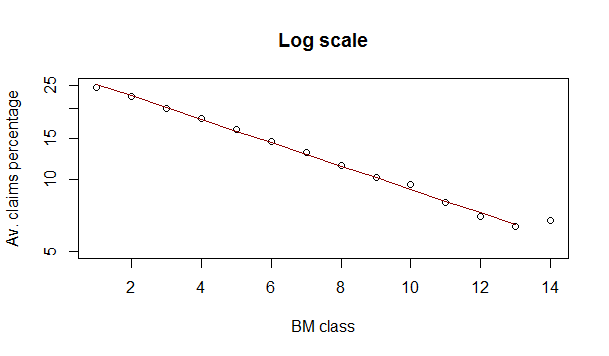
\includegraphics[scale=0.8]{Q15_LogScalePlot.png}

\caption{Log-scale plot of bonus-malus class vs. average number of claims with linear regression fitted on the first 13 bonus-malus classes}
\label{Figure_Question15}

\end{figure}
\end{center}

In the figure the average number of claims is plotted on a log-scale.


\subsection*{Q16}

To determine the linear regression coefficients and produce the required graphs we execute the code given in the question and add code for the determination of the coefficients and graphs to obtain the following output

\begin{verbatim}
> relWt <- ActualWt/ActualWt[1]
> s3 <- tapply(nCl,W, sum) / tapply(Expo,W, sum); s3 <- s3 / s3[1]
> lm(s3~relWt)$coeff
(Intercept)       relWt 
       0.19        0.83 
> lm(log(s3)~0 + log(relWt))$coeff
log(relWt) 
      0.89 
> 
> par(mfrow=c(1,2)) #put figures in a 1 x 2 array
> plot(relWt,s3, main = "Ordinary scale",ylim=c(1,2.5),
+      xlab="Relative Weight", ylab="Av. number of claims")
> lines(relWt,fitted(lm(s3~relWt)),ylim=c(1,2.5),col="darkred")
> 
> plot(relWt,s3, log = "xy", main = "Log-log scale",ylim=c(1,2.5),
+      xlab="Relative Weight", ylab="Av. number of claims")
> lines(relWt,exp(fitted(lm(log(s3)~0 + log(relWt)))),col="darkred")
>
\end{verbatim}

We force the intercept of the log-log regression to be zero by using the code \verb|log(s3)~0 + log(relWt)|. We see that the coefficients produce a regression line equal to the information in the question. The graphs shown in Figure \ref{Figure_Question16} are produced by \verb|R|.
\begin{center}
\begin{figure}[H]

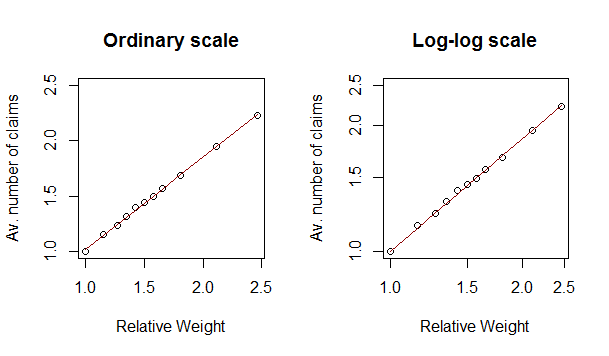
\includegraphics[scale=1]{Q16_OrdinaryAndLogLogScalePlot.png}

\caption{Ordinary scale and Log-log scale plots and regression lines of relative weight vs. average number of claims.}
\label{Figure_Question16}

\end{figure}
\end{center}

\subsection*{Q17}

The young class is defined to be the ages 18-23. If a 18 year old person enters the bonus-malus system in class 5 and does not make any claims he will be in class 10 when 23 years old. Therefore it is impossible to be young and also be in the bonus-malus classes 11-14. \\

The model thus does not support persons in the young age class to be in bonus-malus classes 11-14. Taken together with the other risk factors (\verb|R| has 3 classes, \verb|A| has 3 classes and 1 in calculation, \verb|M| has 3 classes, \verb|U| has 2 classes, \verb|B| has 14 classes and 11-14 in calculation and \verb|WW| has 11 classes) there will be \begin{equation}
3 \times 1 \times 3 \times 2 \times 4 \times 11 = 792 
\end{equation}
empty classes.
\subsection*{Q18}
To determine the loss ratios with respect to the risk groups we use the example code for loss ratios per risk group from page 12 from assignment 2 to obtain the following output.
\begin{verbatim}
> GrandTotalLossRatio <- sum(TotCl)/sum(TotPrem)*100 ## the grand total loss ratio in pct
> GrandTotalLossRatio
[1] 56
> for (rf in list(B,WW,R,M,A,U)) ## for all risk factors, do:
+   {print(round(tapply(TotCl,rf,sum)/tapply(TotPrem,rf,sum)*100))}
 1  2  3  4  5  6  7  8  9 10 11 12 13 14 
53 58 58 59 62 64 63 57 59 62 53 52 50 53 
 1  2  3  4  5  6  7  8  9 10 11 
58 60 58 58 58 57 57 55 56 54 53 
 1  2  3 
56 57 56 
 1  2  3 
58 57 55 
  1   2   3 
119  49  73 
 1  2 
52 67 
> 
\end{verbatim}
We see that the loss ratio of the entire portfolio is 56\%. The tables show how the loss ratio differs per risk factor class for each risk factor independently. To visualize the behaviour in the tables we plot the value of the loss ratio with respect to the risk factor class for each risk factor and add the grand total loss ratio line (see Figure \ref{Figure_Question18}, red line is grand total loss ratio).
\begin{center}
\begin{figure}[H]

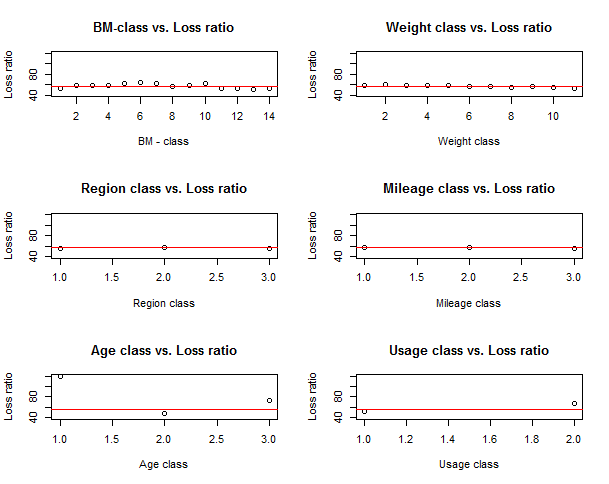
\includegraphics[scale=1]{Q18_Risk_factors_vs_loss_ratio.png}

\caption{Loss ratio vs. Risk factors}
\label{Figure_Question18}

\end{figure}
\end{center}

The annual premium is given in Equation (9.35) of MART
\begin{equation}
\pi_{rambuw} = 500 \times P_b \times (W_w / W_1) \times R_r \times M_m
\end{equation}
where $P_b$ is the factor for the bonus-malus system, $W_w / W_1$ the relative weight factor, $R_r$ the region factor and $M_m$ the mileage factor (factor values per class are given in MART). The premium therefore does not recognise the risk factors age and usage. 

Figure \ref{Figure_Question18} (and the table) clearly show that the loss ratio is very different for the different age groups (Age class vs. Loss ratio). The loss ratio is very high for the young age group, relatively low for the middle age group and again higher for the old age group. This patterns implies that the young and old age class should pay more premium in comparision to the current premium which does not differ by age. Completely rejecting an age class will probably not be possible from a legal perspective because of anti discrimination laws. Asking for a higher premium will be possible for the young age class but will be less socially acceptable for the old age class. Because of these reasons the current situation where the middle age class subsidizes the young and old age class will probably have to remain. \\

Figure \ref{Figure_Question18} (and the table) show that the Usage class vs. the loss ratio gives that Private use (class 1) has a lower loss ratio when compared to Business use (class 2). From a risk perspective it is advisable that this risk factor is incorporated in the rating system. It is probably not advisable to incorporate Usage as risk factor when taking the competitive aspect of the policy into account. Business use usually gives high policy volumes (many policies are sold together) and since the difference in loss ratio is not very large it is not advisable to incorporate usage as a risk factor into the premium. \\

When comparing the loss ratios with respect to BM-classes it can be seen that the first BM-class and the BM-classes 11-14 have lower loss ratios than the average and the other classes have higher loss ratios. The low loss ratio in class 1 is interesting and might be the result of persons which drive more carefull after having filed one or multiple claims. The classes BM-classes 11-14 have large premium discounts because the risk factor in the premium of
\begin{equation}
P_b = 120,100,90,80,70,60,55,50,45,40,37.5,35,32.5,30 \%
\end{equation} 
The discount which gives $37.5 - 30 \%$ of the base premium is not low enough for the performance of the groups 11-14. From a risk perspective it is possible to apply a higher discount. From a market perspective a higher discount is probably unnecessary because of the already low premium in these classes. \\

The comparision of the loss ratios with respect to Region classes shows that the region class are well priced. The loss ratios of $56,57,56$ show that it is not necessary to adjust the premium with respect to the region class. \\

Similarly the comparision of the loss ratio with respect to mileage class shows no great deviation from the average (loss ratios $58,57,55$). From a risk perspective a small recalibration of the mileage discount factors ($90, 100, 110 \%$) is advisable. From a competitive perspective it is probably preferable that the low mileage users pay low premiums. It would be necessary to have more information about the current market placement of the policy whether a small recalibration of the discount factors is advisable. \\

The premium with respect to the relative weight gives that the low weight classes have a higher loss ratio when compared to the higher weight classes. The fit in question 15 already showed that the relationship between the average number of claims and the relative weight is not linear and asking a premium proportional to $w_j^{0.89}$ would be more appropriate. The result of the linearity of the premium with respect to the relative weight is the high loss ratio in the low weight classes and the low loss ratio in the higher classes. The rating system can be improved by changing the premium to 
\begin{equation}
\pi_{rambuw} = 500 \times P_b \times (W_w / W_1)^{0.89} \times R_r \times M_m
\end{equation}

\subsection*{Q19}
We run the code given in the question and obtain
\begin{verbatim}
> l <- list(Use=U,Age=A,Area=R,Mile=M)
> ftable(round(100*tapply(TotCl,l,sum)/tapply(TotPrem,l,sum)),
+        row.vars=2, col.vars=c(1,3,4))
    Use    1                                   2                                
    Area   1           2           3           1           2           3        
    Mile   1   2   3   1   2   3   1   2   3   1   2   3   1   2   3   1   2   3
Age                                                                             
1        111  99  90 108 114 114 114 110  98 143 148 114 209 177 112 155 160 139
2         48  44  41  48  43  40  50  44  40  71  60  55  72  61  52  69  62  56
3         71  65  67  79  75  57  70  64  58  95  86  85 104  93  89  94  82  81
>
\end{verbatim}
The table shows that the middle age group has substantially lower loss ratios than the young and old age groups. In the middle age group the Private use class (usage class 1) has a lower loss ratio than the Business use (usage class 2). The differences in the loss ratio with respect to age and usage classes are to be expected since the premium does not uses these risk factors. \\

The lowest loss ratio (ratio equals 40 \%) can be found in the table where age class equals 2 (middle age class), usage class equals 1 (Private use), area class equals 2 or 3 (town or big city), mileage class equals 3 (high mileage). The highest loss ratio (ratio equals 209 \%) can be found for the young age group, Business use, in a town with low mileage. \\

Since the risk factors mileage and region are already incorporated into the premium the marketing focus should be on the not incorporated risk factors Usage and Age. The marketing focus should be on the middle age class which use their car for Private use. A marketing campaign should simultaneously try to detract the young age class in general and the old age class business users. 


\end{document}
